\section{Observations}
	\subsection{SCA}
	\subsection{Objective}
	% (I) To study the dependence of energy resolution on the applied high voltage and to determine the best operating voltage for the scintillation detector.

	% \subsection{\label{sec:level1}Observation and analysis}
	% \subsubsection{\label{sec:level1}Operating voltage=500v}
	% table.1
	% \begin{table}[h]
	\centering
	\begin{tabular}{|c|c|c|c|}
	\hline
	\textbf{\begin{tabular}[c]{@{}c@{}}Angle\\ $(\theta)$\end{tabular}} & \textbf{Time (s)} & \textbf{Counts} & \textbf{\begin{tabular}[c]{@{}c@{}}Counts per\\ second $N(\theta)$\end{tabular}} \\ \hline
	\multirow{5}{*}{25} & \multirow{5}{*}{600} & 133 & \multirow{5}{*}{0.225} \\ \cline{3-3}
	 &  & 140 &  \\ \cline{3-3}
	 &  & 127 &  \\ \cline{3-3}
	 &  & 137 &  \\ \cline{3-3}
	 &  & 138 &  \\ \hline
	\multirow{5}{*}{20} & \multirow{5}{*}{200} & 164 & \multirow{5}{*}{0.940} \\ \cline{3-3}
	 &  & 198 &  \\ \cline{3-3}
	 &  & 186 &  \\ \cline{3-3}
	 &  & 195 &  \\ \cline{3-3}
	 &  & 197 &  \\ \hline
	\multirow{5}{*}{15} & \multirow{5}{*}{100} & 311 & \multirow{5}{*}{2.929} \\ \cline{3-3}
	 &  & 276 &  \\ \cline{3-3}
	 &  & 277 &  \\ \cline{3-3}
	 &  & 311 &  \\ \cline{3-3}
	 &  & 290 &  \\ \hline
	\multirow{5}{*}{10} & \multirow{5}{*}{100} & 1726 & \multirow{5}{*}{17.626} \\ \cline{3-3}
	 &  & 1811 &  \\ \cline{3-3}
	 &  & 1713 &  \\ \cline{3-3}
	 &  & 1754 &  \\ \cline{3-3}
	 &  & 1809 &  \\ \hline
	\multirow{5}{*}{5} & \multirow{5}{*}{100} & 2931 & \multirow{5}{*}{29.286} \\ \cline{3-3}
	 &  & 2938 &  \\ \cline{3-3}
	 &  & 2912 &  \\ \cline{3-3}
	 &  & 2931 &  \\ \cline{3-3}
	 &  & 2931 &  \\ \hline
	\multirow{5}{*}{-5} & \multirow{5}{*}{100} & 2934 & \multirow{5}{*}{29.343} \\ \cline{3-3}
	 &  & 2933 &  \\ \cline{3-3}
	 &  & 2935 &  \\ \cline{3-3}
	 &  & 2935 &  \\ \cline{3-3}
	 &  & 2935 &  \\ \hline
	\multirow{5}{*}{-10} & \multirow{5}{*}{100} & 1751 & \multirow{5}{*}{17.824} \\ \cline{3-3}
	 &  & 1778 &  \\ \cline{3-3}
	 &  & 1831 &  \\ \cline{3-3}
	 &  & 1787 &  \\ \cline{3-3}
	 &  & 1766 &  \\ \hline
	\multirow{5}{*}{-15} & \multirow{5}{*}{100} & 291 & \multirow{5}{*}{2.940} \\ \cline{3-3}
	 &  & 294 &  \\ \cline{3-3}
	 &  & 289 &  \\ \cline{3-3}
	 &  & 290 &  \\ \cline{3-3}
	 &  & 306 &  \\ \hline
	\multirow{5}{*}{-20} & \multirow{5}{*}{200} & 210 & \multirow{5}{*}{1.009} \\ \cline{3-3}
	 &  & 194 &  \\ \cline{3-3}
	 &  & 211 &  \\ \cline{3-3}
	 &  & 201 &  \\ \cline{3-3}
	 &  & 194 &  \\ \hline
	\multirow{5}{*}{-25} & \multirow{5}{*}{600} & 133 & \multirow{5}{*}{0.225} \\ \cline{3-3}
	 &  & 140 &  \\ \cline{3-3}
	 &  & 127 &  \\ \cline{3-3}
	 &  & 135 &  \\ \cline{3-3}
	 &  & 141 &  \\ \hline
	\end{tabular}
	\caption{Table for $N(\theta)$ for 5mm thick Gold foil}
	\label{tab:1}
\end{table}
	% \begin{figure}[h!]
	% \centering
	% 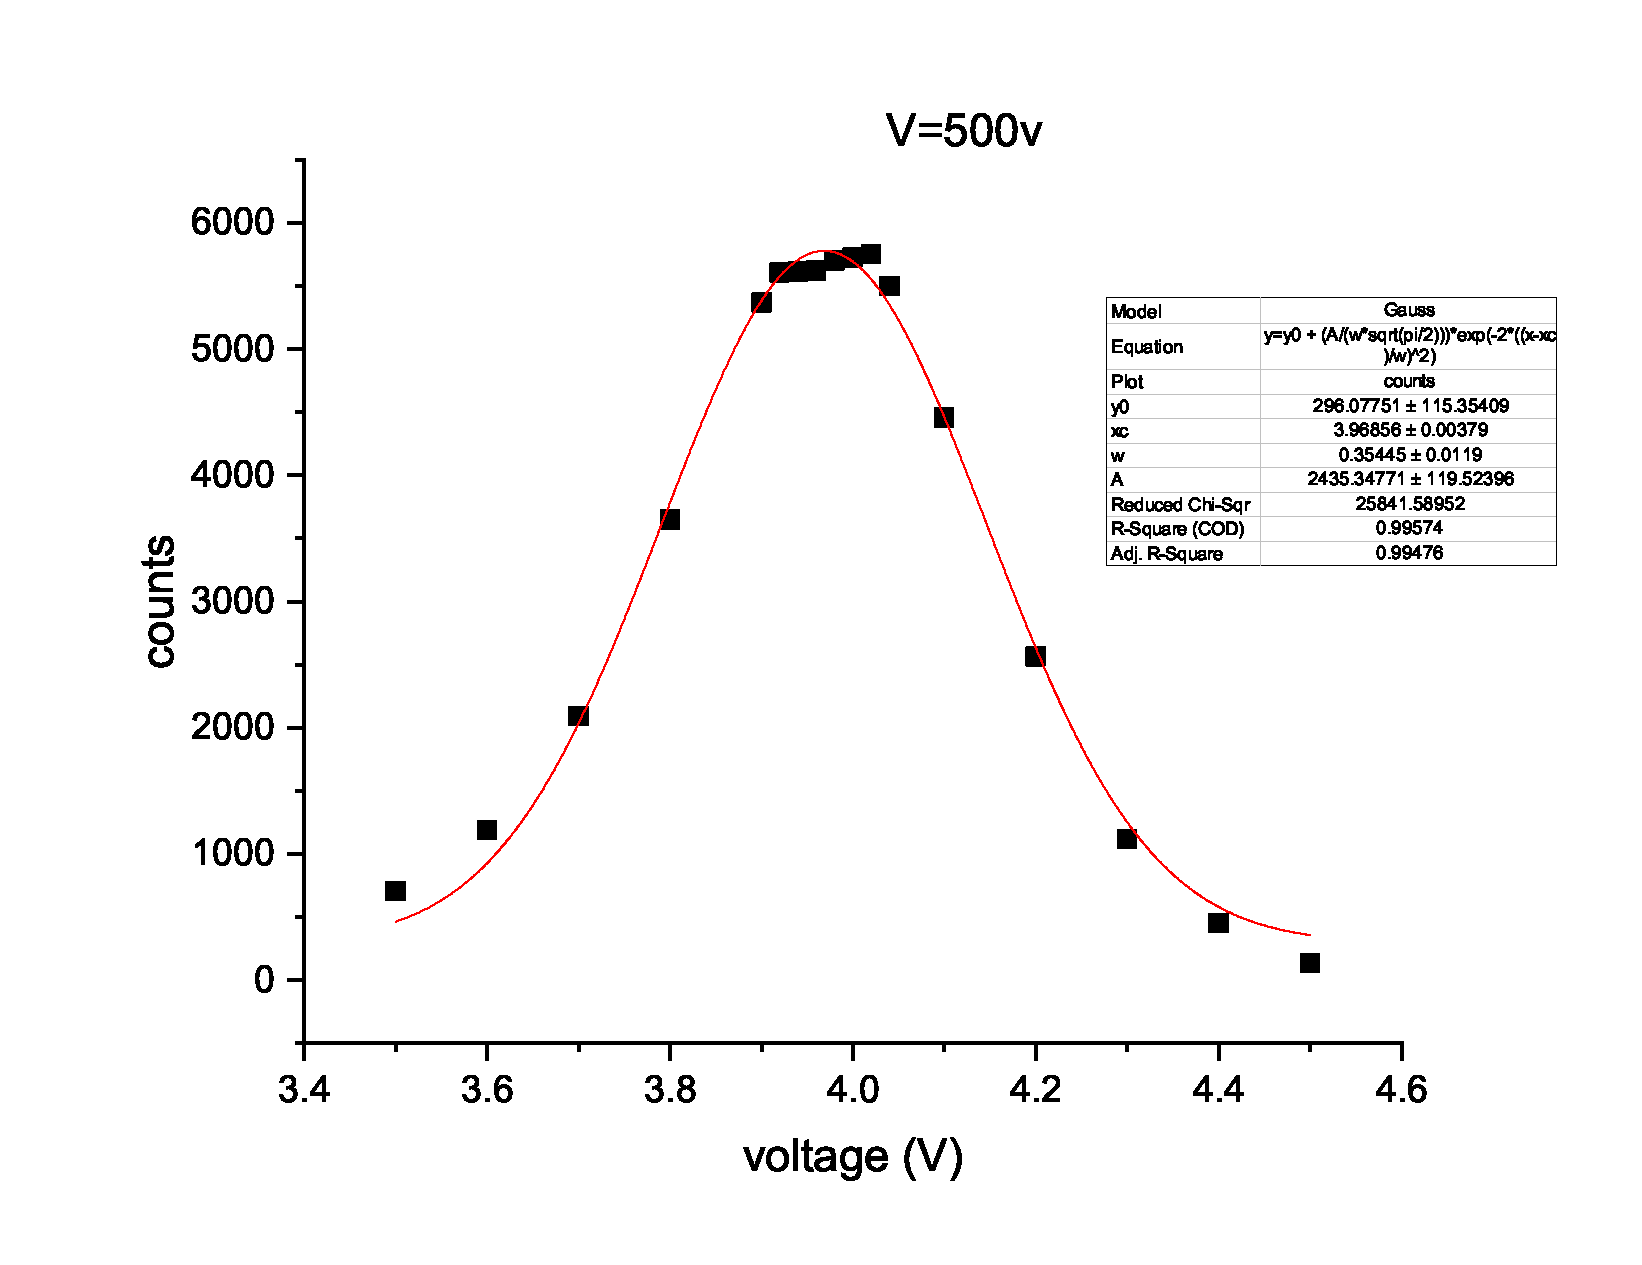
\includegraphics[width=90mm]{Graph1.eps}% Here is how to import EPS art
	% \caption{\label{fig:epsart} V vs counts}
	% \end{figure}
	% \subsubsection{\label{sec:level1}Operating voltage=550v}
	% table.2
	% \begin{table}[H]
    \centering
    \begin{tabular}{|c|c|c|c|}
        \hline
        $V_{DC}$ & $V_{DUT}$ & $V_{OUT}$ & $C_{DUT}$   \\ \hline
        0        & 0.074     & 0.459     & 127.837 \\
        0.1      & 0.109     & 0.451     &  85.276 \\
        0.2      & 0.232     & 0.447     &  39.709 \\
        0.3      & 0.299     & 0.438     &  30.191 \\
        0.4      & 0.389     & 0.432     &  22.888 \\
        0.5      & 0.463     & 0.432     &  19.230 \\
        0.6      & 0.564     & 0.426     &  15.567 \\
        0.7      & 0.662     & 0.420     &  13.075 \\
        0.8      & 0.760     & 0.435     &  11.796 \\
        0.9      & 0.846     & 0.430     &  10.475 \\
        1        & 0.941     & 0.426     &   9.330 \\
        1.1      & 1.058     & 0.427     &   8.318 \\
        1.2      & 1.174     & 0.422     &   7.408 \\
        1.3      & 1.267     & 0.418     &   6.799 \\
        1.4      & 1.357     & 0.416     &   6.318 \\
        1.5      & 1.464     & 0.412     &   5.800 \\
        1.6      & 1.559     & 0.409     &   5.406 \\ \hline
    \end{tabular}
    \caption{Data for light condition}
    \label{tab:2}
\end{table}
	% \begin{figure}[h!]
	% \centering
	% 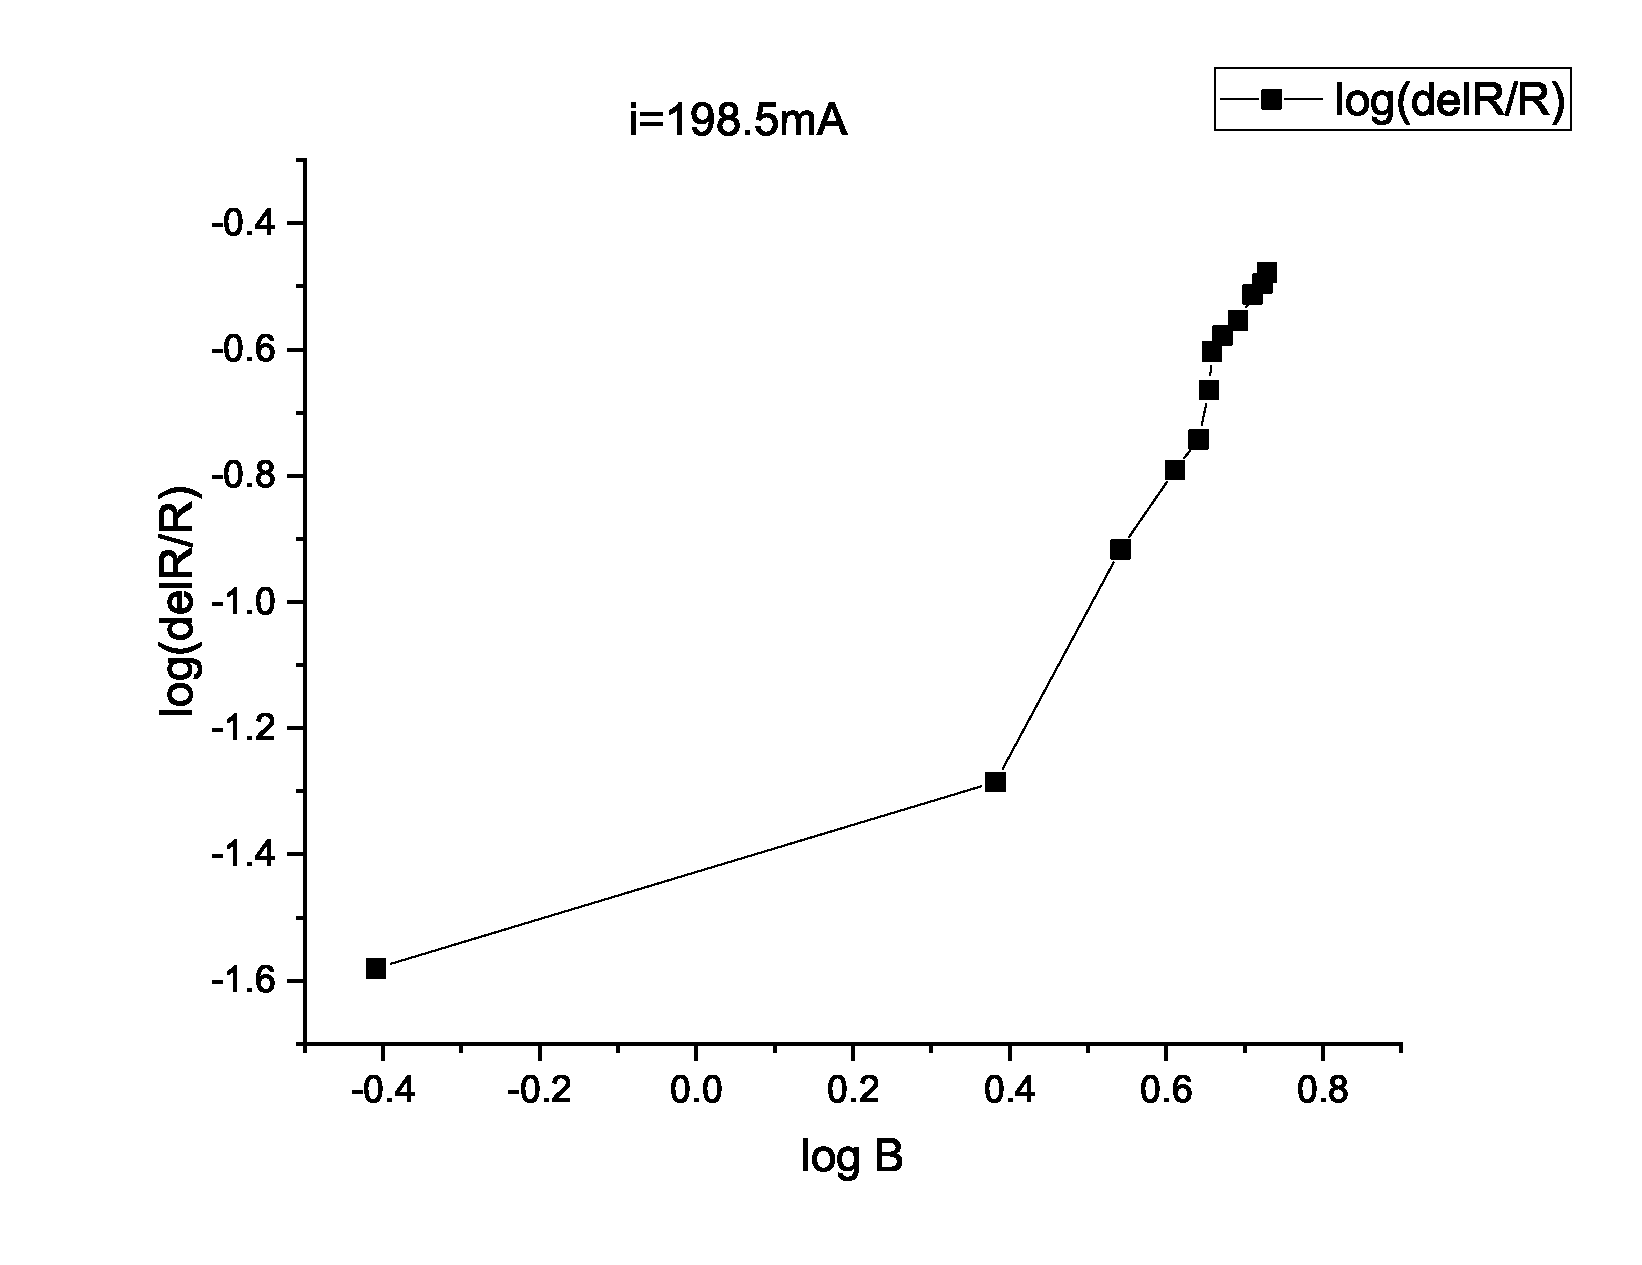
\includegraphics[width=90mm]{Graph2.eps}% Here is how to import EPS art
	% \caption{\label{fig:epsart}V vs counts}
	% \end{figure}
	% \subsubsection{\label{sec:level1}Operating voltage=500v}
	% table.3
	% \begin{table}[]
	\centering
	\begin{tabular}{|l|l|}
	\hline
		H(gauss) & V(mV) \\ \hline
		2390 & -0.061 \\ \hline
		2540 & -0.062 \\ \hline
		3160 & -0.063 \\ \hline
		3480 & -0.064 \\ \hline
		4200 & -0.065 \\ \hline
		4500 & -0.066 \\ \hline
		4780 & -0.067 \\ \hline
		5200 & -0.068 \\ \hline
		5180 & -0.069 \\ \hline
	\end{tabular}
	\caption{Magnetoresistance Data for $I=101.0mA$}
	\label{tab:mag2}
\end{table}
	% \begin{figure}[h!]
	% \centering
	% 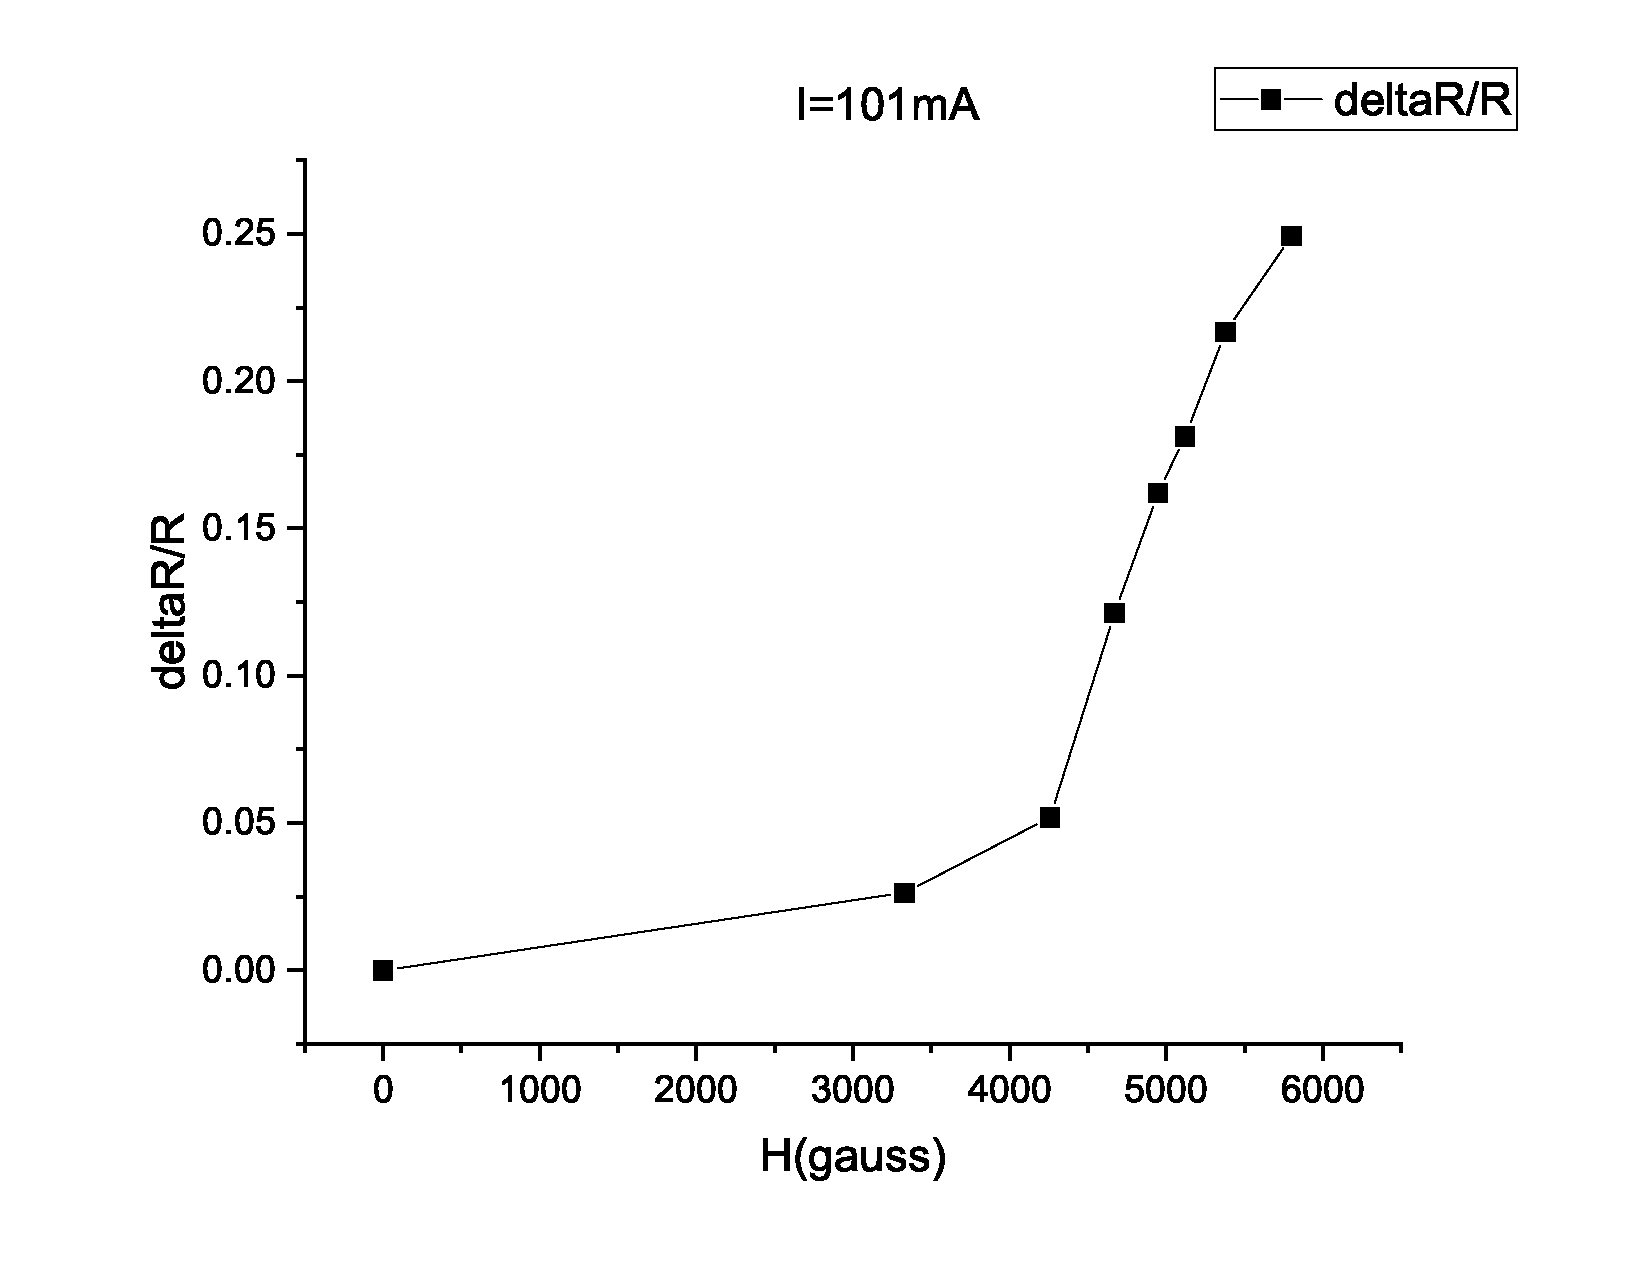
\includegraphics[width=90mm]{Graph3.eps}% Here is how to import EPS art
	% \caption{\label{fig:epsart}V vs counts}
	% \end{figure}
	% \subsubsection{\label{sec:level1}Operating voltage=500v}
	% table.4
	% \begin{table}[h]
	\centering
	\resizebox{\columnwidth}{!}{%
		\begin{tabular}{|c|c|c|c|c|c|}
			\hline
			\textbf{Source}                      & \textbf{Distance (cm)} & \textbf{Counts} & \textbf{Corrected Counts} & \textbf{Average}         & \multicolumn{1}{l|}{\textbf{CPS}} \\ \hline
			\multirow{3}{*}{\textbf{$Cs^{137}$}} & \multirow{3}{*}{10}    & 738             & 655                       & \multirow{3}{*}{670.667} & \multirow{3}{*}{11.178}           \\ \cline{3-4}
			                                     &                        & 766             & 683                       &                          &                                   \\ \cline{3-4}
			                                     &                        & 757             & 674                       &                          &                                   \\ \hline
			\multirow{3}{*}{\textbf{$Tl^{204}$}} & \multirow{3}{*}{2}     & 2306            & 2223                      & \multirow{3}{*}{2224}    & \multirow{3}{*}{37.067}           \\ \cline{3-4}
			                                     &                        & 2309            & 2226                      &                          &                                   \\ \cline{3-4}
			                                     &                        & 2306            & 2223                      &                          &                                   \\ \hline
		\end{tabular}%
	}
	\caption{Efficiency Data}
	\label{tab:4}
\end{table}
	% \begin{figure}[H]
	% \centering
	% 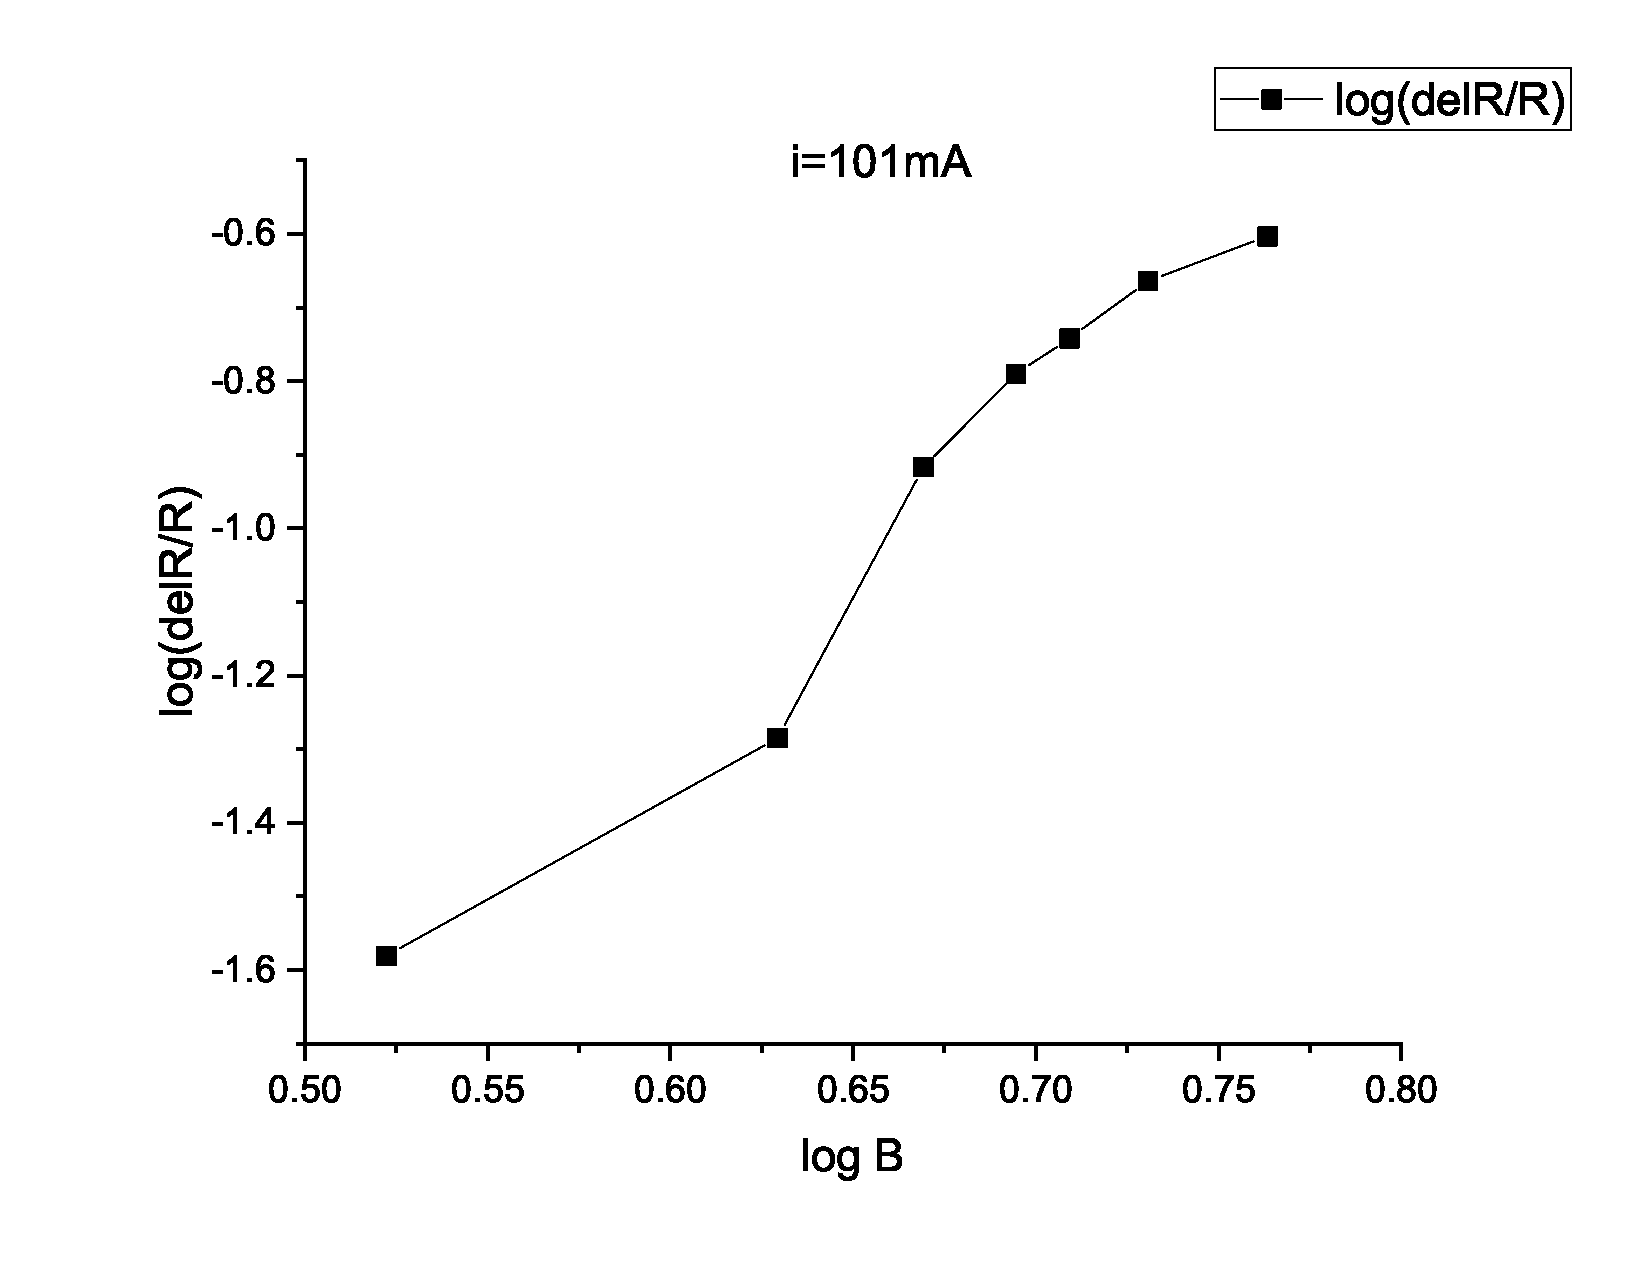
\includegraphics[width=90mm]{Graph4.eps}% Here is how to import EPS art
	% \caption{\label{fig:epsart}V vs counts}
	% \end{figure}
	% \subsubsection{\label{sec:level1}Summary}
	% table.4
	% \begin{table}[H]
    \centering
    \begin{tabular}{|l|l|l|l|}
    \hline
        Operating voltage & ~ & FMWH & Resolution(\%) \\ \hline
        500 & ~ & 0.41734 & 10.38 \\ \hline
        550 & ~ & 0.39714 & 10.18 \\ \hline
        600 & ~ & 0.3943 & 10.48 \\ \hline
        650 & ~ & 0.40354 & 10.29 \\ \hline
    \end{tabular}
    \caption{Operating voltage vs FMWH and resolution}
    \label{tab:resolution}
\end{table}
	% \begin{figure}[H]
	% \centering
	% 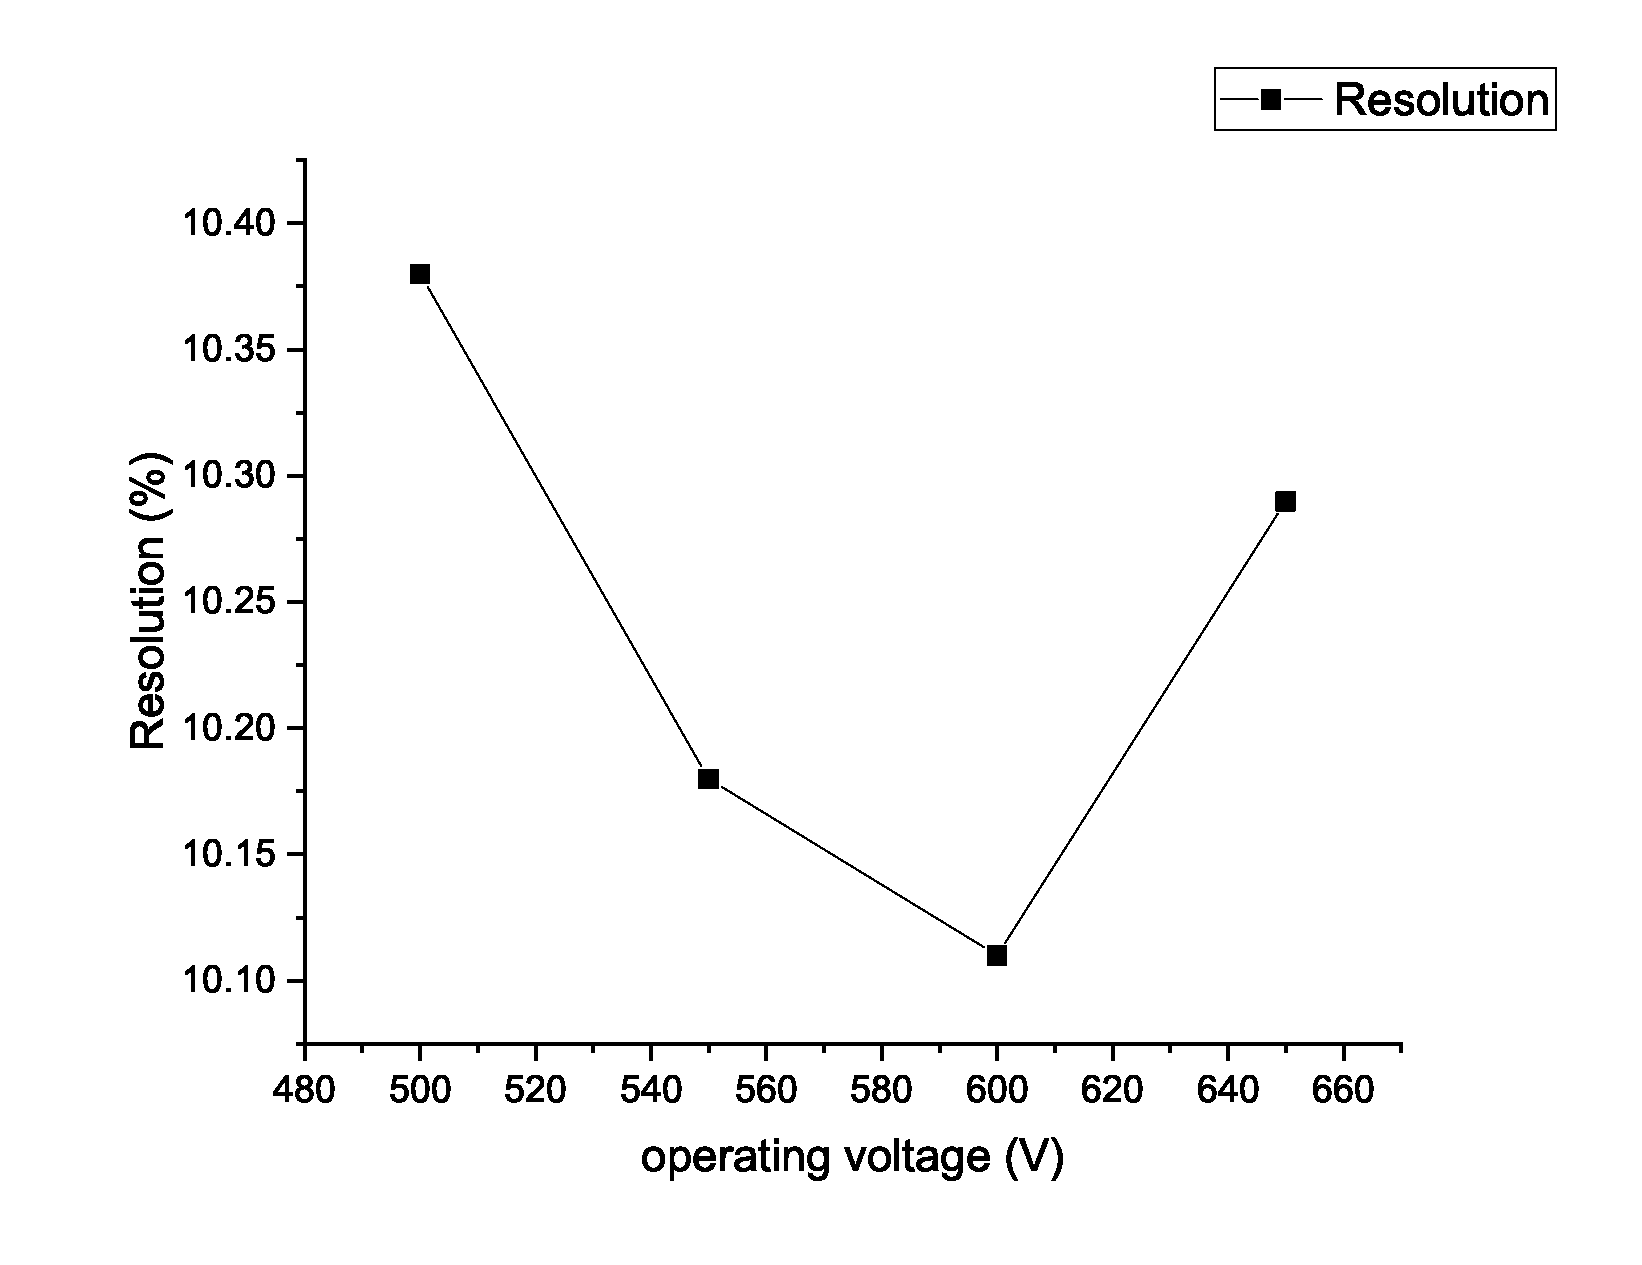
\includegraphics[width=90mm]{Graph5.eps}% Here is how to import EPS art
	% \caption{\label{fig:epsart}V vs counts}
	% \end{figure}\\
	% Thus from Fig.5 we have an operating voltage as 600v with a resolution of 10.11\%.
